\documentclass[preprint,authoryear,12pt]{elsarticle}
\PassOptionsToPackage{hyphens}{url}\usepackage{hyperref}
\usepackage{amssymb}
%\usepackage{amsmath}
\usepackage{pslatex}
\usepackage[overlap,CJK]{ruby}
\usepackage{linguex}
%\usepackage[pdftex]{graphicx}
\usepackage{graphicx}
\usepackage{multirow}
\usepackage{subfigure}
\usepackage{paralist}
%\usepackage{setspace}

\newcommand{\hlc}[2][yellow]{ {\sethlcolor{#1} \hl{#2}} }

%\renewcommand{\baselinestretch}{1.5}
\date{}
\pagestyle{empty}

\usepackage{color}
\usepackage{soul}

 \topmargin0mm
 \headheight0mm
 \headsep0mm
 \oddsidemargin0cm
 \textwidth15.5cm
 \textheight23cm

%% a useful little macro for comments and notes
\newcommand{\MNOTE}[1]{\marginpar{\tiny\raggedright\em #1}}
\setlength{\marginparsep}{2.2pt}
\setlength{\marginparwidth}{40pt}
%%\newcommand{\MNOTE}[1]{}
\newcommand{\Dutchvon}[2]{#2}

\setcounter{secnumdepth}{4}
%\newcommand{\comment}[1]{{\color{blue}{#1}}}
%\newcommand{\commenthp}[1]{{\color{red}{#1}}}
%\newcommand{\subsubsubsection}[1]{\paragraph{#1}\mbox{}\\}

\makeatletter
\renewcommand{\paragraph}{\@startsection{paragraph}{4}{\z@}%
  {-3.25ex\@plus -1ex \@minus -.2ex}%
  {1.5ex \@plus .2ex}%
  {\normalfont\normalsize\mdseries}}
\renewcommand{\subparagraph}{\@startsection{subparagraph}{5}{\z@}%
  {-3.25ex\@plus -1ex \@minus -.2ex}%
  {1.5ex \@plus .2ex}%
  {\normalfont\normalsize\bfseries}}
\makeatother



% Select what to do with todonotes:
\usepackage[disable]{todonotes} % notes not showed
%\usepackage[draft]{todonotes}   % notes showed

% Select what to do with command \comment:
\newcommand{\commentHidden}[1]{}  % my "private comments", are invisible in PDF.
\newcommand{\previous}[1]{}


%\newcommand{\theme}[1] {\par {\bfseries \color{blue} #1 \par}} %the theme of paragraph or section showed in blue
%\newcommand{\question}[1] {\par {\bfseries \color{red} #1 \par}} % the question posed to the Prendinger sensei is showed in Red
%\newcommand{\commentShow}[1] {\par {\bfseries \color{orange} #1 \par}} % my "public" comments shown in orange! This may describe, what I am thinking or seeking



\newcommand{\myChange}[1] {\par {\color{brown} #1 \par}} % my "public" comments shown in orange! This may describe, what I am thinking or seeking




% When in final version, to hiden all the themes, questions, comments etc, commend the above command lines and uncomment the following lines


\newcommand{\theme}[1] {} %the theme of paragraph or section showed in green
\newcommand{\question}[1] {} % the question posed to the sensei is showed in Red
\newcommand{\commentShow}[1] {} % my "public" comments shown in Green! This may describe, what I am thinking
\newcommand{\plagiarism}[1]{}




\begin{document}

\begin{frontmatter}
\title{Large-Scale Data Collection of Eco-Driving Behavior:
Analysis of a Campaign with the iCO$_2$ Simulation Platform}

\author[label1]{Helmut Prendinger}
\author[label1]{Raghvendra Jain}
\author[label2]{Daniela Fontes}
\author[label2]{Henrique T. Campos}
\author[label2]{Hugo M.C. Damas}
\author[label1]{Anjie Fang}
\author[label1]{Zhi Qu}
\author[label1]{Bernd Hollerit}
\author[label2]{Rui Prada}


%\author[label3]{Klaus Br\"ugmann}

\address[label1]{{helmut@nii.ac.jp, jain@nii.ac.jp, fanganjie@gmail.com, hollerit@gmail.com, zq12721@my.bristol.ac.uk}\\
	National Institute of Informatics, \\
    2-1-2 Hitotsubashi, Chiyoda-ku, Tokyo, 101-8430, Japan\\}

\address[label2]{{danielafilipa@gmail.com,henriquetcampos@gmail.com,hugo.damas@gmail.com,rui.prada@tecnico.ulisboa.pt}\\
    INESC-ID and Instituto Superior T\'{e}cnico, Universidade de Lisboa,\\
    Av. Prof. Cavaco Silva, Taguspark Porto Salvo, Portugal\\}

%\address[label3]{{mail@klausbreugmann.de}\\
%	??? \\
%	Tokyo, Japan\\}

\begin{abstract}
We describe iCO$_2$,\footnote{The first six authors equally contributed to this paper.} a simulation platform for collecting driving behavior data. For the user, iCO$_2$ is designed as a massively multiplayer online game for mobile devices to practice eco-friendly driving. For the researcher, iCO$_2$ constitutes a Human Computation system that facilitates the collection of large-scale data on driving behavior to better understand \hl{compliance and} incentive mechanisms for eco-driving and users' preferences. The main contribution of the paper is \hl{two-fold}. First, we describe the newest version of our iCO$_2$ simulation platform, which has been extended to a game with a quest system and functions to upgrade the player's vehicle. Second, we present the results of a campaign with iCO$_2$ that uses a game promoter to attract more than 3000 users in a short time. Our game run on servers in Asia, Europe and America.
\hl{The results are described from three angles: (1) types of drivers are identified by clustering driving behavior; (2) types of players are identified by relating of players' interaction with game elements and their driving behavior; (3) by looking a longer sessions, we demonstrate that players who show eco-unfriendly behavior at the beginning of the session improve over their playtime.}
\end{abstract}

\begin{keyword}
Data collection; data analysis; driving behavior; Human Computation system; Games with a Purpose; massively multiplayer online game
\end{keyword}

\end{frontmatter}

%%%%%%%%%%%%%%%%%%%%%%%%%%%%%%%%%%%%%%%%%%%%%%%%%%%%%%%%%%%%%%%%%%%%%
% INTRODUCTION
%%%%%%%%%%%%%%%%%%%%%%%%%%%%%%%%%%%%%%%%%%%%%%%%%%%%%%%%%%%%%%%%%%%%%
\section{Introduction and Motivation}\label{sec:intro}

%Testing references:
%\citep{Andrade+others.2005,Bellotti+others.2009,Hwang+Salvendy.2010,Csikszentmihalyi.1990}
%\cite{Andrade+others.2005,Bellotti+others.2009,Hwang+Salvendy.2010,Csikszentmihalyi.1990}


Our world today is tightly interconnected by the Internet, which allows users from almost anywhere to access information anytime in an affordable and immediate manner. For scientists, this situation opens hitherto unknown opportunities for experimental testing of novel online applications. While in principle vast populations can  be reached quickly and effortlessly, motivating users to participate in social experiments is a big challenge. It is important to provide an adequate incentive other than money to the users, so that they do not have any motivation to cheat \citep{Quinn}.
As a solution, Games With a Purpose (GWAP) have been proposed \citep{vonAhn2006Games}. GWAP is a field of Human Computation \citep{Yuen.2009,Krause+Smeddinck.2011} that seeks to motivate users, such as annotators of pictures or testers of applications, through enjoyment rather than any monetary incentive.

The recent rise of mobile devices---such as smart phones, tablet computers or handheld game consoles---has opened up new opportunities to conduct experiments beyond laboratory studies. Ubiquitous computing access makes it possible to reach large numbers of users, although it is more difficult to standardize test conditions, and control the environment.
\cite{Henze2013} \hl{suggested a ten-step-program to conduct large-scale studies with mobile applications in order to obtain valuable data that cannot be collected in a lab setting: (1) clearly identify the research goals; (2) select a study method; (3) devise an incentive mechanism;  (4) choose the target platform(s); (5) design and develop the mobile app; (6) prepare data collection; (7) implement a scheme to obtain informed consent from users; (8) distribute and promote the app; (9) continuously monitor data collection for a designated time period; (10) filter and analyze data to answer the research question.}

In this paper, \hl{we adhere to these steps} and present iCO$_2$, a massively multiplayer online (MMO) driving game. iCO$_2$ is designed as a mobile application that allows players to practice eco-friendly driving. Eco-driving is a term used to describe the usage of vehicles in an energy efficient way, such as smooth acceleration and deceleration, keeping the speed limit, and so on.

Notably, iCO$_2$ is a platform for collecting driving behavior data and in-game decision data from users. It can be accessed as an app on ``Google play``.\footnote{https://play.google.com/store/apps/details?id=net.globallabproject.ico2\&hl=en}
Our data collection platform uses a hybrid strategy to give an incentive to players, which is based on (1) a mobile games promoter to attract players to the game and (2) in-game mechanics to keep them playing. We use Tapjoy\footnote{http://home.tapjoy.com/}, %\citep{TapJoy}
a company that handles mobile games promotion, to attract a large number of users (in the 1000s) to iCO$_2$ within a short time. This approach constitutes an alternative to the tools and applications that have been used in research projects involving games \citep{kittur2008crowdsourcing,Biewald:2012,ChanH12}.
To keep players motivated, we provide a quest system and the possibility to upgrade the user's car as in-game mechanics.

The main \hl{research contribution} of this paper is a human-computer study with a driving simulator that
\begin{itemize}
\item shows to what extent our eco-driving interface supports eco-driving behavior, i.e., compliance to straightforward eco-driving principles such as smooth acceleration and deceleration;
\item investigates the relationship between in-game driving behavior and other in-game behavior, such as visiting the ``Garage'', where users could upgrade and modify their car with the in-game money rewarded from the quests; and
\item describes how the driving behavior of users in the simulated environment evolves over time.
\end{itemize}


The paper is structured as follows.
Section \ref{sec:background} provides background research on eco-driving games, training applications, crowdsourcing and games with a purpose.
Section \ref{sec:platform} describes the iCO$_2$ simulation platform that extends our previous version of iCO$_2$
\citep{prendingeroliveira2014} with a quest system and upgrade functions.
In Section \ref{sec:campaign} we explain the campaign and present usage statistics of iCO$_2$ during the campaign.
Section \ref{sec:result} presents the results regarding driving behavior types and player types.  Moreover we test the hypothesis that iCO$_2$ players tend to become better at eco-driving.
Section \ref{sec:conclusions} summarizes and discusses the most relevant results and describes future work.

%The appendix contains additional tables in \ref{app:tables} and the list of abbreviations in \ref{app:abbreviations}.

%%%%%%%%%%%%%%%%%%%%%%%%%%%%%%%%%%%%%%%%%%%%%%%%%%%%%%%%%%%%%%%%%%%%%
% RELATED WORK
%%%%%%%%%%%%%%%%%%%%%%%%%%%%%%%%%%%%%%%%%%%%%%%%%%%%%%%%%%%%%%%%%%%%%	
\section{Related Work}\label{sec:background}

In this section, we will first report on eco-driving games and training applications.
%and analyze how iCO$_2$ differs by involving a massively multiplayer element, a mobile distribution method and a three dimensional (3D) environment.
Then we will explain how our work can be positioned within the crowdsourcing literature.

\subsection{Eco-driving Games and Training Applications}
\label{subsec:eco-driving}

The training of eco-driving is important as it greatly affects world-wide fuel expenditure and pollution emissions \citep{barkenbus2010eco,shaheen2012ecodriving}. Therefore, car manufacturers have started to develop applications that provide drivers with some feedback on the effects of their driving behavior \citep{EcoTools,FiatEcoGame}.

%iCO$_2$ is \question{first and foremost} an eco-driving game. It has been designed to work as a massive multiplayer online (MMO) game. Therefore it is possible that users interact with each other, as they would in real life driving. It has been designed to be played in mobile systems so that it is as  accessible as possible by the masses. In particular, our target audience are gamers; a group that has seen its size and playtime exponentially grow over recent years \citep{MobileStats}.


%\question{It is important to note that the player is not the only one who receives feedback on his or her  driving. Our underlying data gathering system can provide important information to future developers of iCO$_2$ on how to improve the design of the eco-driving simulator.} \commentShow{needs to be re-written.}

%The aforementioned qualities make iCO$_2$ stand out from any other eco-driving application in the industry. \commentShow{Really ? It's just an opinion, not an academic claim. }

Most applications for practicing eco-friendly driving are either 2D single-player games \citep{EcoGame1, EcoGame2, TruckEcoGame, Moebius, FiatEcoGame} or full-fledged simulators that can only be played with specific physical apparatus \citep{EcoSimulator, GreenDino, EcoSimulator2, sabrina2013enhanced}. By contrast, iCO$_2$ is a massively multiuser 3D game that can be controlled by common mobile devices.

%While there are MMO driving games, none of them allows users to keep track of the effect of their driving behavior on their fuel consumption and gas emissions. And while there are applications, even games, which incorporate the aforementioned features, none of them are MMO driving games.

\subsection{Crowdsourcing and Games with a Purpose}
\label{subsec:csandgwap}

We have defined our project as a Human Computation system \citep{Yuen.2009,Krause+Smeddinck.2011}, rather than a crowdsourcing system.
\cite{Quinn} explain the difference comprehensively. The most important distinction is that crowdsourcing involves the entire problem being tackled by a crowd of humans \citep{howe2008crowdsourcing}, whereas Human Computation involves only part of a problem being tackled by a crowd of humans.

Our goal is to collect and discern driving behavior in a simulated environment. Our users fill in for a part of the ``algorithm'' of data collection, which involves them ``providing behavior''.
%Our game neatly adheres to the definitions of Games With a Purpose given by \cite{Quinn} and \cite{vonAhn2006Games}, albeit with a slightly more ambiguous problem definition: to collect real-time behavioral driving data from users.

More specifically, our game fits the definition of Games With a Purpose given by \cite{Quinn} and \cite{vonAhn2006Games}, which is explained as an area in the field of Human Computation that aims to use enjoyment as a primary means of motivating users.
To draw users of our game, we initially provide a a monetary incentive. Our method to provide the system with users is based on Tapjoy,\footnote{https://home.tapjoy.com/} a games promoter. Tapjoy works by offering mobile gamers in-game rewards for whatever game they are currently playing, in exchange for engaging with another game, such as our iCO$_2$.


\subsubsection{Crowdsourcing}

%\cite{Biewald:2012} and \citep{ChanH12} introduce systems that might be related to ours; however, they do not involve GWAP.

\cite{Biewald:2012} presents a number of applications involving crowdsourcing and Human Computation that use the increasingly popular Mechanical Turk from Amazon \citep{MechTurk} and involve ethics, business and fun. The tasks involve answering questions that don't require any technical knowledge or performing Google searches. ``Sifu`` by \citep{ChanH12} is a system that supports language learning by providing tutoring services to readers of news sites and articles. The crowd is recruited from an online social network instead of using the Mechanical Turk.

We note that while these two applications use distinct sources of ``crowds for hire``, they are acquiring a group of users to participate in their research by performing specific tasks that constitute the experiment as a whole. This further illustrates why we consider iCO$_2$ a Human Computation system: iCO$_2$ is not meant to rely on hiring a crowd to do a (particular) job, but rather to play a game, have fun and practice eco-driving. As a side effect, the crowd provides data about their behavior.

However, our (research) goal does not necessarily motivate the crowd of users. This is where Games with a Purpose come into play.

\subsubsection{Games with a Purpose}

iCO$_2$ is a Game with a Purpose: data collection. In particular, we are interested in driving behavior data and data about the players' in-game behavior.

\cite{vonAhn:2004} introduced the concept of GWAP with the now well-known ESP game, which had the aim to label images. Here, players are matched and have to guess which label their counterpart is applying to the image that both of them are seeing. Subsequently, the project was improved and re-branded as Peekaboom \citep{vonAhn:2006} and Phetch \citep{vonAhn:2007}.

%KissKissBan \citep{Ho:2009} extended on previous approaches of player matching by integrating cooperative and competitive elements into a game with the purpose of annotating images. One player tries to make it so a pair of other players can't agree on a description about an image, which not only adds a cheating-proof mechanism but also promotes diversity of image annotations. Even later, these concepts were extended with more functionality by another team with their game Karido \citep{steinmayr2011karido}.

%These applications are successful in improving image databases. They focus on labeling, description, information (knowing what objects an image contains), and keyword/tag diversity (by providing similar images, so users are forced to choose differentiating keywords/tags), respectively. However, even with being played by a massive crowd of players, user interaction is always on a small scale: one to one.

%\paragraph*{Audio tagging -- TagATune}

A similar approach to the previously outlined image tagging endeavors is taken with TagATune \citep{Law:2009}, a game with a purpose that also matches players online one-to-one. They play a game of tagging a piece of music that may or may not be shared by the two and when they are offered each other's music and tags, they try and guess if it is indeed the same sound sample or not. The game resurfaced with the modified intent of gauging the success of machine-run algorithms that tag music \citep{vonAhn&Law:2009}.

%\paragraph*{User preference -- Matchin}

%Matchin \citep{Hacker:2009} is a GWAP that follows the same gameplay flow as ESP but instead of tagging, each player has two images and has to try and guess which one will be preferred by the matched player. The goal is to gather information on user preference for an image database.

%\paragraph*{Location tagging -- EyeSpy}

%EyeSpy \citep{Bell:2009}, more of a social networking endeavor, motivates players to tag locations with descriptions, and then others to confirm them, by having a point system and a ranking. Meanwhile, the system retrieves a collection of recognizable geographic details that can be used towards supporting navigation tasks. Notably, EyeSpy is available on web-browsers and mobile applications, akin to iCO$_2$.

%\paragraph*{Collecting common sense facts \& goals -- Verbosity, CommonConsensus}

%Verbosity \citep{vonAhnVerb:2006} and CommonConsensus \citep{lieberman2007}, while having different purposes, are both web-based knowledge games where players play via the browser to select an answer to given questions that is considered more or less correct. They are given a question and choose an answer they expect strangers to give. The more frequently an answer is given, the more correct it is considered. There is no user-to-user interaction in the case of these two applications besides interacting with the knowledge produced by the masses (which includes them). Verbosity sought to collect facts that were commonsense while Common Consensus sought to collect goals.

%\paragraph*{Prediction of protein structures -- Foldit}

Foldit \citep{cooper2010predicting} puts players in a puzzle-solving game involving the prediction of protein structures. By providing online functionalities such as chatting or ranking, they keep their players engaged with both difficulty and socialization. Chatting and ranking are functionalities iCO$_2$ does not provide at this point, because we believe those features would distract from the core functionality and purpose of the game.

%\paragraph*{Behavioral data -- Caretaker}



\subsubsection{Comparison of previous Games with a Purpose to iCO$_2$}

Caretaker \citep{Violi:2011} is a project that notably focuses on behavioral data, and the analysis thereof, that pertains to trust. Caretaker places four players in a board-like game that simulates a transport square-shaped network across which they have to travel from corners to center. Three players must ally against the fourth and arrive at the center before this common enemy, despite none of the three knows who the adversary is when the game starts. Their position in the network is the only publicly available information but the game offers a chat system to communicate as they wish. Violi et al. also logged player actions as a method through which they can match and confirm the behavioral information they receive from having the players submit a survey.

Caretaker has many similarities to iCO$_2$ as a Human Computation system: the player's actions and decisions are logged in order to analyze behavioral data.
%and the users are playing with and against each other, which approximates real behavior. However, we posit that the goal of the ``bad`` player is to be the enemy of the other three, while the goal of the other three is to find out who their friends are. If they know who is who, they can cooperate to win.
In iCO$_2$, the situations are potentially much more akin to real life circumstances, with drivers just encountering other motorists they know nothing about, and choosing how to interact with them based on the same variables that would influence them in a real scenario (situation, mood, etc). There is also the massive multiplayer element to iCO$_2$, which Caretaker does not have.

%When regarded as a whole, there is no research project quite like iCO$_2$.
%iCO$_2$ has followed in the footsteps of previous Games with a Purpose, applying proven and time-tested strategies, but on a large scale in a previously untouched area of study.


iCO$_2$ follows some design decisions used in previous Games with a Purpose. Challenge is cited as a key factor for a successful game \cite{vonAhn.2008}, in the game design we tried to add mechanisms such as resource management (fuel, car characteristics), to create a more challenging experience. Multiplayer experiences, time-sensitive decisions, randomness are also characteristics mentioned in \cite{vonAhn.2008}, that can improve the enjoyment and we used in the design of iCO$_2$.

iCO$_2$ constitutes a Human Computation system, because we want to collect driving behavior and decision information from a massive quantity of users, while training them on eco-driving and providing them with enjoyment and fun.

%\subsection{Analysis of Driving Data in Simulated Environments}

\section{The iCO$_2$ Data Collection Platform}\label{sec:platform}

The iCO$_2$ game is a massively multiuser online driving simulator that provides players with a tool to practice eco-driving (see Figure~\ref{fig:iCO2_driving}). In the game, players drive in a 1km$^2$ replica of Tokyo city, whereby streets are populated both with other players' cars and with computer controlled cars from our traffic simulator system \citep{Prendinger+others.2014}. As a result, traffic situations occur naturally in the virtual environment, which can be utilized to investigate eco-driving policies \citep{Prendinger+others.2013} or traffic congestion \citep{Gajananan+others.2013}.

iCO$_2$'s predecessor version \citep{prendingeroliveira2014} contained two game modes, (1) ``Free drive'' and (2) ``Campaign'', where players are paid for completing a quest or task. By contrast, the current version of iCO$_2$ offers a full-fledged quest system, and hence players can engage in repeated campaign-style interactions.

By completing quests, players are rewarded with virtual currency (within the iCO$_2$ game), which is the key factor that motivates players to maintain eco-driving behaviors. Fuel-efficient driving reduces the amount of fuel spent when completing a quest and thereby saves in-game money. If the players manage to save sufficient in-game money, they are able to upgrade their car with components that improve eco-efficiency.

\begin{figure}[htb]
\begin{center}
\includegraphics[width=.95\linewidth]{ijhcs14-img/iCO2_driving}
\caption{Screenshot of the iCO$_2$ game, which displays a player driving around the replica of Tokyo city. On the top-left, the car's velocity and fuel consumption information is displayed. The acceleration/break slider is located on the right.\label{fig:iCO2_driving}}
\end{center}
\end{figure}


\subsection{Feedback on Eco-driving Mechanisms}

The game provides players with visual information about the car's fuel/energy consumption. As shown on the top-left of Fig.~\ref{fig:iCO2_driving}, the interface displays instant consumption, 10 seconds consumption, 60 seconds consumption, and overall consumption. The timed consumption elements change colors according to the players' eco-efficiency. Green indicates eco-efficiency whereas read indicates eco-inefficiency.

The implementation of the input controller for acceleration and breaking was an important design decision. As opposed to many other driving simulators, which feature a single button for acceleration and another button for breaking, we considered an option for a smooth change of pace tantamount; it should feel like using pedals in a real car. In order to achieve these nuances, we decided to provide a slider (shown on the right side in Figure~\ref{fig:iCO2_driving}), which lets users accelerate, decelerate and maintain constant speeds easily. For the mobile application, this feature was realized by touch controls, while the web player could be operated via mouse.


\subsection{Quests}
\label{subsec:quests}

The quest system in iCO$_2$ is a mechanism to motivate players to stay in the simulation environment. Each quest consists of a sequential set of legs. In each leg, the player has to transport passengers and/or cargo from a start point to a destination. When a player starts a quest, the first leg is triggered and only after that leg is completed the next one will be activated. While driving, the player can identify the legs' start and finish points as hovering arrows, as shown in Fig.~\ref{fig:iCO2_driving}.

Quests are dynamically generated so that the player always sees multiple simultaneous quests. In that way, the game allows players to carefully plan their route before driving. The player also has to manage the car's accommodations, e.g.~to increase the number of seats for passengers or space for cargo.

\subsection{Garage}

With the in-game money rewarded from quests, players can go to the \textit{Garage} and upgrade their car with advanced technology (see Fig.~\ref{fig:iCO2_garage}). By upgrading the car, the players can enhance their car's eco-friendliness. Further, the player can buy a new car that features different configurations, such as engine power, mass, capacity to carry passengers and cargo, etc. Players are also able to customize their car by selecting a different color.

When a player owns more than one car, it is up to him or her to decide which car to use for a quest. Hence a player is able to choose between a car that have more passenger or cargo capacity, but high fuel consumption, or a car with a small capacity but less fuel consumption.


\begin{figure}[htb]
\begin{center}
\includegraphics[width=.80\linewidth]{ijhcs14-img/iCO2_garage}
\caption{Screenshot of the iCO$_2$ \textit{Garage}, where the player can buy new vehicles and upgrades as well as repaint the owned cars.\label{fig:iCO2_garage}}
\end{center}
\end{figure}

\subsection{Navigator}

In the game, players can use the in-game \textit{Navigator} system (see Fig.~\ref{fig:iCO2_navigator}) to enhance their route planning. This tool guides the players in the game's scenario by displaying their cars' current position and the current start and finish points of the active quests' legs. Players can zoom in/out the map to better understand the street layout.

Moreover, while driving, players are guided towards the legs' start and finish points by an augmented reality arrow (see Fig.~\ref{fig:iCO2_driving}). The arrow points players to the direction they have to follow to reach the start and destination points to the quests' legs.

\begin{figure}[htb]
\begin{center}
\includegraphics[width=.95\linewidth]{ijhcs14-img/iCO2_navigator}
\caption{Screenshot of the \textit{Navigator} tool, which guides the player in the virtual scenario. The player's car is represented with the car icon. Blue icons represent the legs' start points, red icons mark the legs' end points. The arrows connect the origin to the destination.\label{fig:iCO2_navigator}}
\end{center}
\end{figure}



\subsection{Implementation}

The game was developed with the Unity3D game engine\footnote{www.unity3d.com}, which allows us to seamlessly port the iCO$_2$ game to different platforms. The game can currently be played on mobile devices (Android and iOS) and in web browsers via the Unity web player. The game is available in English and Japanese.

The multiplayer feature of iCO$_2$ is enabled by DiVE (Distributed Virtual Environments) \citep{prendingeroliveira2014}. DiVE handles the communication among all the iCO$_2$ components (see Figure~\ref{fig:iCO2_generalarchitecture}), which we regard as DiVE clients.

Each client works as follows: The ``Profile Client'' handles the persistency of the players' profile. Players' profiles are associated to their Facebook accounts. Therefore, players do not need to perform any additional registration to iCO$_2$ and always retrieve their progress regardless of the platform that he/she is using to play the game. The ``Spawn Client'' manages where players spawn when they enter the game's scenario. With this system, we are able to distribute players evenly throughout the map. The ``Logging Client'' retrieves players' driving data, such as the car's position, velocity, etc., and stores it persistently in a database. The ``Traffic Simulator'' system controls the computer-controlled cars and all traffic lights in the virtual scenario.

\begin{figure}[htb]
\begin{center}
\includegraphics[width=.6\linewidth]{ijhcs14-img/iCO2_generalarchitecture}
\caption{iCO$_2$ system architecture. The DiVE server supports the communication platform between all the different components that compose the iCO$_2$ system. The left side shows the clients, in different platforms, controlled by the player. The right side shows the clients that support the iCO$_2$ system.\label{fig:iCO2_generalarchitecture}}
\end{center}
\end{figure}

%\section{Methodology}\label{sec:2campaigns}




\section{A Campaign with the iCO$_2$ Simulation Platform}\label{sec:campaign}

%In our international campaign, 7073 users played the iCO$_2$ game. We discarded the data of users who played less than 3 minutes, leaving us with statistics of 1562 players.

In March 2014, we run a campaign with iCO$_2$ for one week and collected data of 3184 mobile users. The results of our data analysis will be discussed in the following sections.


%In our experiment (see Section~\ref{sec:campaign}), we motivated users to try our game in that way: Tapjoy requires them to spend a certain amount of time in the game environment, after which only the enjoyment factor could keep them engaged.

\subsection{Implementing the Campaign}
\label{subsec:campaign}

In our large-scale study, we aimed to follow the ten-step framework proposed in \citep{Henze2013}.
The {\itshape first step\/} relates to identifying the research goals clearly. The objective of our study is to collect and analyze data on the eco-driving behavior of users in a simulated city environment. Besides understanding player types and in-game behavior, we also wanted to investigate whether our eco-feedback mechanism improves eco-driving over time. The {\itshape second step\/} is to devise a study method, such as correlational or experimental. This work focuses on correlational research to identify phenomena, including correlation between player type and interaction with game elements, or the evolution of eco-driving behavior over a time period. We used the games promoter Tapjoy to attract users ({\itshape third step}). For the time of the performing the requested task (two quests), the incentive as extrinsic, users earn `points' that can be used as in-game currency in the game the user played before joining the campaign. However, after the completion of the task, we can be assumed that some intrinsic incentive (`fun') prevails.
The target platform chosen for this study was Android smartphones and tablets ({\itshape fourth step}). Regarding the {\itshape fifth step}, iCO$_2$ is designed as an engaging application that supports data collection at scale. We track the player's position every 100ms and record it in our log server, along with other behavioral information ({\itshape sixth step}). Users login with their Facebook accounts and consent to the term of data usage upon a prompt from the application ({\itshape seventh step}). Regarding the ({\itshape eighth step}), we distribute the application via Google Play, and the games promoter Tapjoy.
The Tapjoy campaign ran for a week, during each we monitored the servers and database to ensure the system was functioning ({\itshape ninth step}). The we processed and analyzed the data ({\itshape tenth step}).

In Section \ref{sec:result}, we present our analysis and insights from our experiment. First, we report on the usage statistics.


\subsection{Usage Statistics}
\label{subsec:usage_stats}

Figures \ref{fig:engagement}, \ref{fig:completion}, \ref{fig:4diagrams_color}, \ref{fig:4diagrams_transactions},  \ref{fig:time} and the Tables \ref{T:Activityswitch_all} and \ref{T:Carswitch_all}  show different usage statistics of the iCO$_2$ campaign. A `quest' in iCO$_2$ encompasses the activity of picking up a passenger or cargo at a starting point and bringing (delivering) the passenger (cargo) to a destination. For both activities, the player has to completely stop the car. In our campaign, the task of the users was to complete two quests.
`Engagement' is a term used by Tapjoy and refers to the requirement of receiving a reward. In our case, players had to complete two quests.

\begin{figure}[htb]
	\begin{center}
		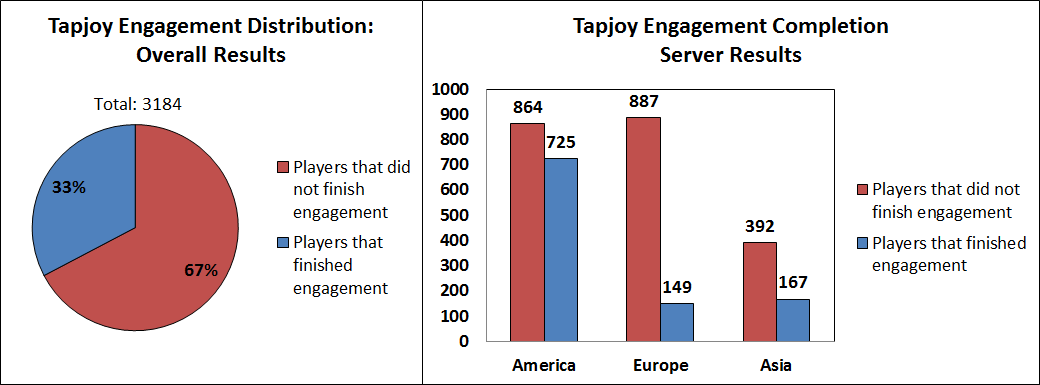
\includegraphics[width=.95\linewidth]{ijhcs14-img/engagement}
		\caption{iCO$_2$ statistics: Engagement.\label{fig:engagement}}
	\end{center}
\end{figure}

\begin{figure}[htb]
	\begin{center}
		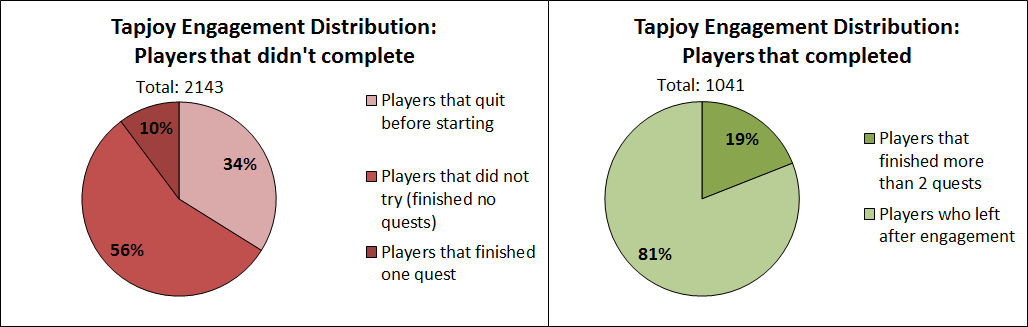
\includegraphics[width=.95\linewidth]{ijhcs14-img/completion}
		\caption{iCO$_2$ statistics: Completion.\label{fig:completion}}
	\end{center}
\end{figure}


%\begin{figure}[htb]
%	\begin{center}
%		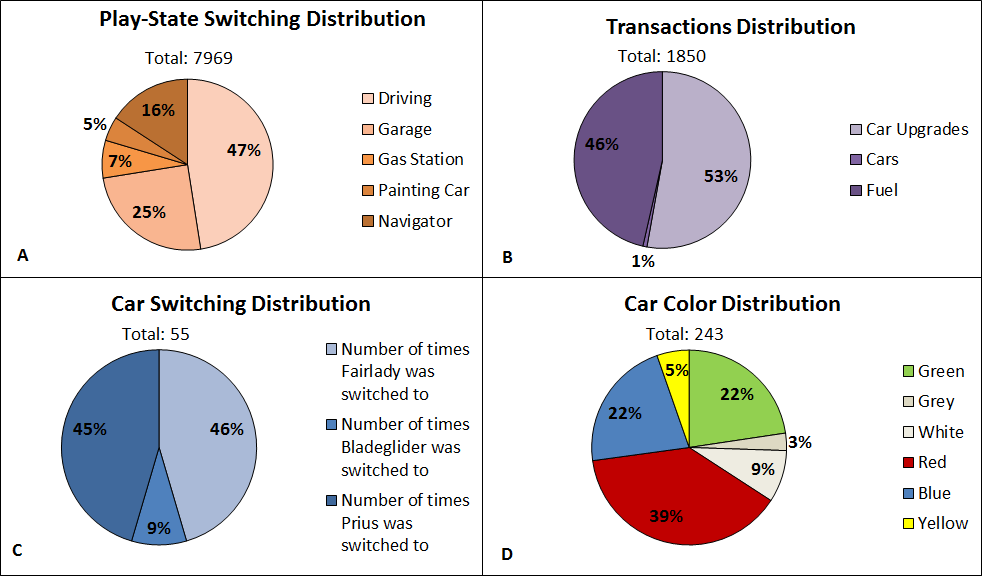
\includegraphics[width=.95\linewidth]{ijhcs14-img/4diagrams2}
%		\caption{Various iCO$_2$ statistics.\label{fig:4diagrams}}
%	\end{center}
%\end{figure}

\begin{figure}[htb]
	\begin{center}
		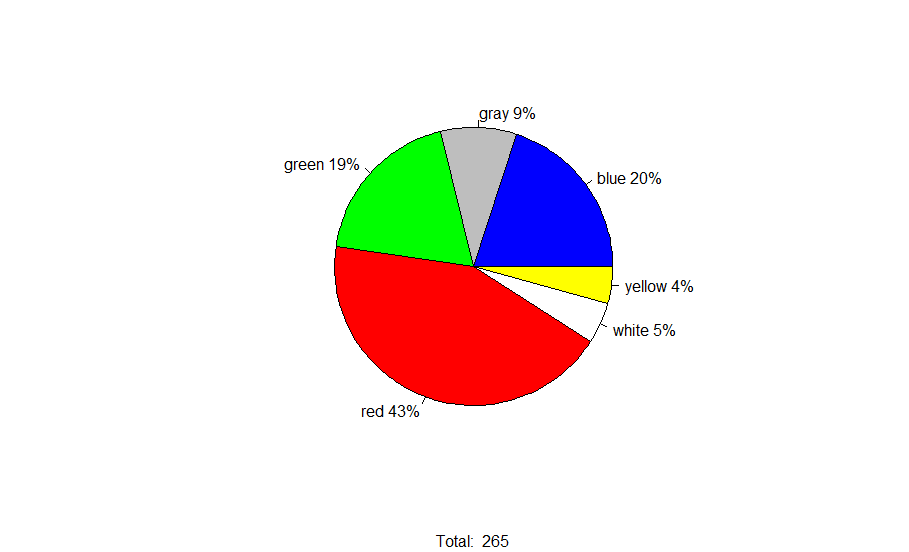
\includegraphics[width=.95\linewidth]{ijhcs14-img/colour_all}
		\caption{Car color distributions for the players that switched car color.\label{fig:4diagrams_color}}
	\end{center}
\end{figure}

\begin{figure}[htb]
	\begin{center}
		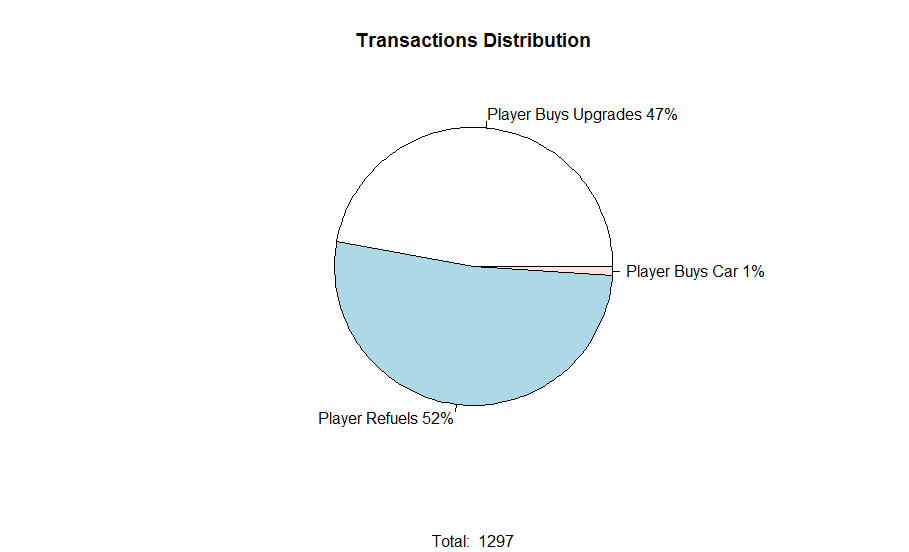
\includegraphics[width=.95\linewidth]{ijhcs14-img/transactions_all}
		\caption{Transactions distribution.\label{fig:4diagrams_transactions}}
	\end{center}
\end{figure}

\begin{table}[!htb]
	\renewcommand*{\arraystretch}{1.4}
	\caption{This table presents the activity switched during the game.}
	\begin{center}
		\begin{tabular}{c|c|c|c|c|c|c}
			Current Activity/ Next Activity & CarPainter & Driving & Garage & GasStation &  Navigator\\
			\hline
			CarPainter & 0&	348&	0&	1&	0\\
			
			Driving & 10&	0&	1971&	566&	1257\\
			
			Garage& 356&	1472&	0&	4&	9\\
			
			GasStation& 0&	524&	20&	0&	6\\
			
			Navigator& 0&	1258&	0&	0&	0\\
			
			
		\end{tabular}
	\end{center}
	\label{T:Activityswitch_all}
\end{table}







\begin{table}[!htb]
	\renewcommand*{\arraystretch}{1.4}
	\caption{This table presents the car switches performed by all players.}
	\begin{center}
		\begin{tabular}{c|c|c|c}
			Current Car/ Switched Car & Prius & Fairlady & BladeGlider \\
			\hline
			Prius &	 0
			& 24  & 3  \\
			
			Fairlady & 9
			& 0  &  2 \\
			
			BladeGlider &	 0
			& 1  &  0  \\
			
		\end{tabular}
	\end{center}
	\label{T:Carswitch_all}
\end{table}


In total, 3184 players have played iCO$_2$; among them, 33\% finished the engagement (see Fig.~\ref{fig:engagement}). American players had the highest participation and completion rate, with 725 players finishing the engagement, while 864 did not. European users were most likely to abandon the engagement, with 887 players not finishing and only 149 completing the engagement. 392 Asian users, who were mostly from Japan, did not finish the engagement while 167 did.

Figure \ref{fig:completion} shows the number of players that did not complete the engagement. Out of a total of 2143 users that did not finish the engagement, 10\% of players finished one quest, 34\% quit before even starting, and 56\% did not try to finish a quest. In total, 1041 users completed the engagement, 81\% left after the engagement and 19\% finished more than two quests.


The number of times a player logs into the game helps us to better understand the way players interact with iCO$_2$, or its re-playability potential. A `play session' is an uninterrupted chunk of play time. The majority of players only played the game once, as we can see on Figures \ref{fig:playtime_e}, \ref{fig:playtime_as}, and \ref{fig:playtime_a} (in Appendix).
On the Europe server, 21.7\% of the players opened the game at least twice; that number is 18.8\% for Asia, and 10.2\% for America.

We can see various iCO$_2$ statistics in 
%Fig.~\ref{fig:4diagrams}
Figures \ref{fig:4diagrams_color}, \ref{fig:4diagrams_transactions}, and the Tables \ref{T:Activityswitch_all} and \ref{T:Carswitch_all}. 
Tables \ref{T:Activityswitch_all} shows the play-state switching distribution, Figure \ref{fig:4diagrams_transactions} shows the transaction distribution, Table \ref{T:Carswitch_all} shows the car switching distribution, and Figure \ref{fig:4diagrams_color} shows the car color distribution. The play-state was switched a total of 7802 times, mostly towards the driving state. In Figure \ref{fig:4diagrams_transactions}, we can see how users spent their in-game currency. Most of it was spent on car upgrades (47\%) and refueling (52\%), with only 1\% spent on new cars. A total of 1297 transactions were made. Users did not switch their cars very often, only a total of 39 switches occurred as denoted in Table \ref{T:Carswitch_all}. As for the color distribution, the users preferred a red car by far (43\%), followed by green and blue (19\% and 20\%) and the less popular white (5\%), yellow (5\%) and grey (9\%). In total, cars were recolored 265 times.

\begin{figure}[htb]
	\begin{center}
		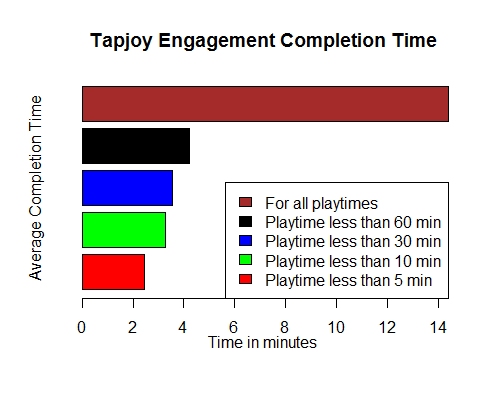
\includegraphics[width=.6\linewidth]{ijhcs14-img/time}
		\caption{ The average engagement completion time for different categories of players. The categorization is done on the basis of whether players finish the engagement (doing atleast 2 quests) in less than a certain threshold time. These categories contains mutually non-exclusive set of players.\label{fig:time}}
	\end{center}
\end{figure}


The average time to complete an engagement is shown in Figure \ref{fig:time}. The engagement task was designed so it could be easily completed under 5 minutes.
However when we look at Figures \ref{fig:playtime_e}, \ref{fig:playtime_as}, and \ref{fig:playtime_a} we can observe that there are players who needed much longer to complete the engagement, and even across multiple play sessions. Moreover for every server, the median is set around the 4 minute mark. This brought us to consider some outlier groups when studying the time that took for each player to complete the two quests.
If we deem all times over 60 minutes outliers, the average engagement completion time drops off to 4 minutes and 23 seconds. It further diminishes to 3 minutes and 53 seconds, if we consider all times over 30 minutes as outliers, to 3 minutes and 26 seconds with outliers over 10 minutes and to 2 minutes and 45 seconds, if we ignore all times over 5 minutes.

In terms of car color, the main difference between the users that finished the engagement and the general population is an increased preference for the color gray in detriment for the color yellow, as we can observe in Figure \ref{fig:engagementcolor}.

\begin{figure}[htb]
	\begin{center}
		\includegraphics[width=.95\linewidth]{ijhcs14-img/Color}
		\caption{Car color distribution for the users that finished the engagement.\label{fig:engagementcolor}}
	\end{center}
\end{figure}

The players who finished the engagement seem to have bought more upgrades in relation to refueling. This can make us hypothesize that these players are more interested in exploring the game.
Given the fact that very player starts off with a Prius, we can see that Fairlady was the most popular car choice. Players did not switched car very often, as we can see in Table \ref{T:Carswitch}, and players who completed the engagement were those who actually switched cars, with 6 switches happening before they complete the engagement. 
These players seem to partake in every game activity, and as expected from the transactions graph in Figure \ref{fig:engagementtransactions}, trips to the garage are more common than trips to the Gas Station.
On average the users who completed the engagement played for more 10 minutes, and did an average of 2.1 more quests.

\begin{figure}[htb]
	\begin{center}
		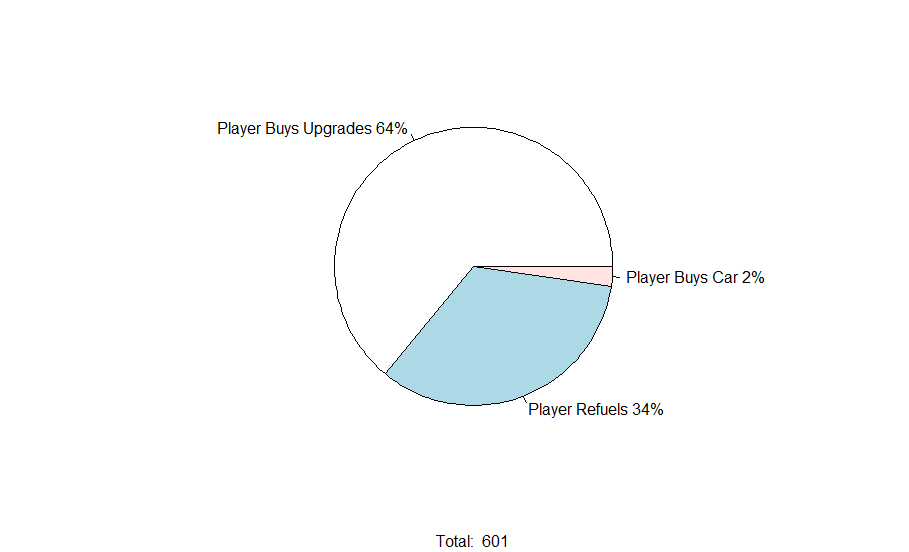
\includegraphics[width=.95\linewidth]{ijhcs14-img/Transactions}
		\caption{Transactions distribution for the users that finished the engagement.\label{fig:engagementtransactions}}
	\end{center}
\end{figure}


\begin{table}[!htb]
	\renewcommand*{\arraystretch}{1.4}
	\caption{This table presents the car switches performed by player who completed the engagement.}
	\begin{center}
		\begin{tabular}{c|c|c|c}
			Current Car/ Switched Car & Prius & Fairlady & BladeGlider \\
			\hline
			Prius &	 0
			& 24  & 3  \\
			
			Fairlady & 3
			& 0  &  2 \\
			
			BladeGlider &	 0
			& 1  &  0  \\
		
		\end{tabular}
	\end{center}
	\label{T:Carswitch}
\end{table}


\begin{table}[!htb]
	\renewcommand*{\arraystretch}{1.4}
	\caption{This table presents the activity switched during the game for player who completed the engagement.}
	\begin{center}
		\begin{tabular}{c|c|c|c|c|c|c}
			Current Activity/ Next Activity & CarPainter & Driving & Garage & GasStation &  Navigator\\
			\hline
			CarPainter &	0&	39&	0&	0&	0\\
			
			Driving & 0	 & 0&	199&	102&	372\\
			
			Garage& 41&	143&	0&	1&	2 \\
			
			GasStation& 	0&	99&	2&	0&	2 \\
			
			Navigator& 0&	375&	0&	0&	0 \\
			
		\end{tabular}
	\end{center}
	\label{T:Activityswitch}
\end{table}



\section{Results}
\label{sec:result}

\subsection{Measurement of Eco-friendliness of Driving Behavior}
\label{sec:measureEco}

The eco-friendliness of a player's driving is measured in terms of acceleration averaged over time.  The car's position is recorded every 100 milliseconds. According to the positional information, speed (the magnitude of the velocity) and average acceleration (the magnitude of the acceleration) is calculated using Equation \ref{eq:velocity}:

\begin{equation}\label{eq:velocity}
Speed(i) = \frac{distance(i,j)}{i-j}
\end{equation}

where $distance(i,j)$ is calculated by the Euclidean distance. $i$ and $j$ represent two neighboring time-stamps. The average acceleration is calculated by Equation \ref{eq:acceleration}:

\begin{equation}\label{eq:acceleration}
Acceleration(i) = \frac{Speed(i) - Speed(j)}{i-j}
\end{equation}

For each user, the time-stamp associated with the speed and average acceleration is logged into the database for the entire duration of driving. In the data, the acceleration of the car is between $-$4 m/s$^2$ and 4 m/s$^2$ most of the time, and the total range is set from $-$6 m/s$^2$ and 6 m/s$^2$.  We define smooth acceleration (and deceleration) as the characteristic of eco-driving and calculate the rate of change of acceleration, i.e., jerk between the two consecutive time-stamps using Eq.~\ref{eq:slope_acceleration}:

\begin{equation}\label{eq:slope_acceleration}
jerk(i) = \frac{Acceleration(i) - Acceleration(j)}{i-j}
\end{equation}

As in \cite{prendingeroliveira2014}, we define 22 categories for the jerk defined in Eq.~\ref{eq:slope_acceleration},
starting with $[-inf , -100]$ up to $[100, +inf]$. Giving these categories smooth acceleration is defined as the $[-10, 0]$, and $[0, 10]$ intervals.

For each player, we first calculate the probability of jerk distributed over the 22 intervals and then normalize the probability distribution of jerk.
After that, an unsupervised machine learning method called clustering which is used to group data into different groups, where data from the same group has similar characteristics and data from different groups is dissimilar.
In our work, $k$-means clustering is used \citep{KMEAN.1979} to determine different driver types and their characteristics. The sum of squares due to error (SSE) is calculated to determine the optimal number of clusters and their convergence.  The smaller the SSE, the better the cluster. The SSE is calculated by Eq.~\ref{eq:sse}

\begin{equation}\label{eq:sse}
SSE = \sum\limits_{i=1}^{k} \sum\limits_{x \in C_{i}}distance(m_{i},x)
\end{equation}

We analyzed $k$ from 2 to 15 and selected the $k$ according the elbow criterion \cite{Thorndike.1953} that achieves a low SSE, while using the least amount of clusters in order to explain the data. To evaluate the eco-friendliness level of these clusters, we introduce Eq.~\ref{eq:factor-accel-slope}

\begin{equation}\label{eq:factor-accel-slope}
factor_{eco} = F_{r[-10,10]}
\end{equation}

which corresponds to the relative frequency of the smooth acceleration bin. The closer this factor is to 1, the more eco-friendly the cluster is.


\subsection{Types of Drivers}

In this section, we show how we identified different driver types based on their driving behavior. First, players who played less than four minutes are filtered out. For the remaining players, driving behavior data is analyzed for the entire driving time, except for the first two minutes that are considered as training time.
Using the `elbow' heuristic to minimize the sum of squares due to error (Equation~\ref{eq:sse}), four clusters are created as shown in Fig.~\ref{fig:accel-ranges}.
Eco-driving is determined by the relative frequency of smooth acceleration in the interval $[-10,10)$. Drivers in Cluster 1, ``crazy'' drivers, have a low presence in the smooth acceleration category, and performed more abrupt brakes and steep acceleration.
Clusters 2 and 4 have a high prevalence of smooth acceleration, whereby drivers in Cluster 2 focus primarily on smooth braking, and drivers in Cluster 4 focus on smooth accelerating; hence, we call them group ``eco-braker'' drivers and ``eco-accelerator'' drivers, respectively. Finally, we have a group of players that perform mostly smooth accelerations but still show abrupt acceleration changes. We label this group as ``normal'' drivers.

\begin{figure}[tb]
	\begin{center}
		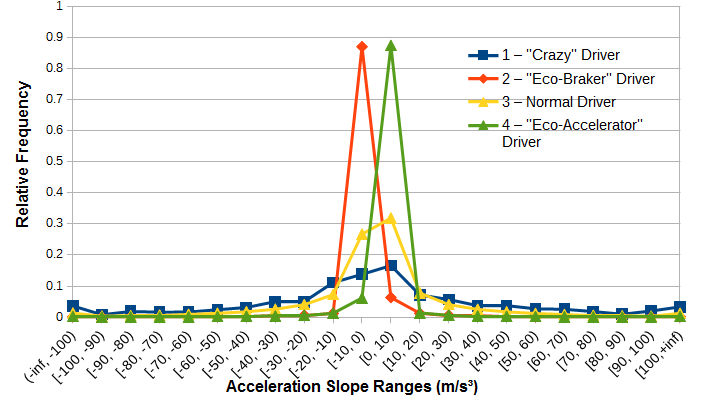
\includegraphics[width=1\linewidth]{ijhcs14-img/kmeansclustering}
		\caption{Clustering of users' driving behavior based on the rate of change of acceleration. \label{fig:accel-ranges}}
	\end{center}
\end{figure}

%sorted table
\begin{table}[!htb]
	\renewcommand*{\arraystretch}{1.4}
	\caption{This table presents a summary of the clusters. Here we present the relative frequency of smooth acceleration for each cluster; the $factor_{eco}$. Moreover the majority of players fits the ``Normal'' driver profile with a considerable amount of smooth acceleration, mixed with abrupt changes. The percentage of users classified as ``Crazy`` (8.08\%) is less that the sum of the two eco-friendly clusters (``Eco-Brakers`` and ``Eco-Accelerators``), combined. }
	\begin{center}
		\begin{tabular}{c|c|c|c}
			Cluster & $factor_{eco}$ & \% of Users & Cluster Label \\
			\hline
			1 &	 0.30
			& 8.1  & ``Crazy`` Driver  \\
			
			2 & 0.93
			& 7.6  &  ``Eco-Braker`` Driver \\
			
			3 &	 0.59
			& 73.1  &  ``Normal'' Driver  \\
			
			4 & 0.94
			& 11.2  &  ``Eco-Accelerator`` Driver \\
		\end{tabular}
	\end{center}
	\label{T:factors}
\end{table}

Detailed results for the clusters are shown in Table \ref{T:factors}.
Please note that the cluster for ``normal'' drivers aggregates the vast majority of the drivers and shows an intermediate percentage of time on the smooth acceleration interval (59\%).

The users who finished the engagement did not seem to strive away from the proportions obtained when performing the clustering analysis, which can be seen in Table \ref{T:factors}. The main difference being that the presence of ''Crazy Drivers'' seems to be more accentuated.

\begin{figure}[tb]
	\begin{center}
		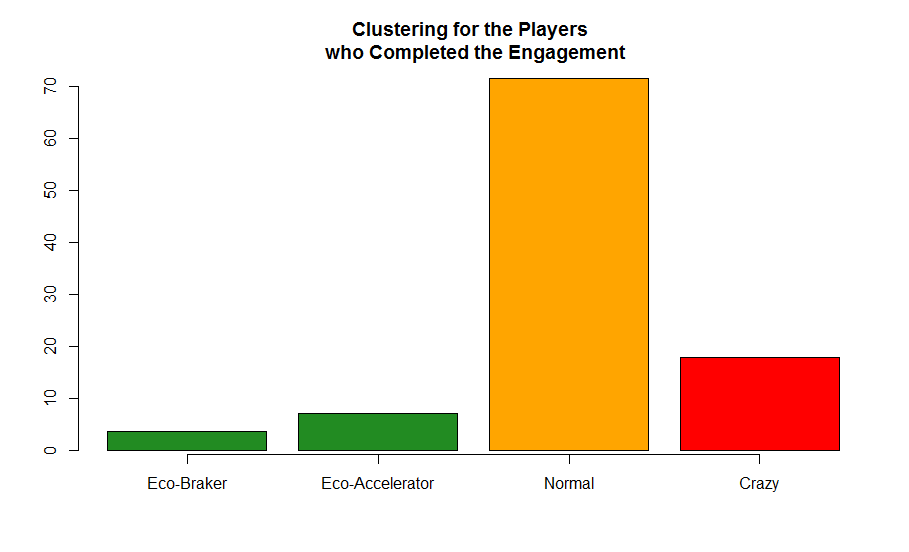
\includegraphics[width=1\linewidth]{ijhcs14-img/Rplot01}
		\caption{Results of the cluster classification on the users that finished the engagement. \label{fig:clusteringengagement}}
	\end{center}
\end{figure}

\subsection{Types of Players}

After we classified users according to their driving behavior, we were curious how their driving behavior might affect other in-game activities, i.e., what types of {\em players\/} there are.

First, we are interested in the correlation between painting a car in a particular color and being an ``eco-unfriendly'' driver.\footnote{In the real world, such information can be interesting for insurance companies.}
``Eco-unfriendliness'' is characterized by the levels of the $factor_{eco}$ parameter in Table \ref{T:factors}. This enables us to order our clusters from the most to the least eco-friendly cluster: Cluster 4 $<$ Cluster 2 $<$ Cluster 3 $<$ Cluster 1, or ``Eco-Accelerator``  $<$ ``Eco-Braker`` $<$  Normal $<$ ``Crazy``.

We use Kendall correlation coefficient to find associations between the data, which enables us to understand the relationship between the ranks of the variables. Kendall correlations provide a number between -1 and 1. A negative correlation coefficient means that it is negatively correlated, in this case, it means more eco-friendly users tend to do a certain behavior. When we have a positive correlation, it means that a certain behavior is associated with being more eco-unfriendlt, given our cluster ordering: ``Eco-Accelerator``  $<$ ``Eco-Braker`` $<$  Normal $<$ ``Crazy``.  We performed this analysis for every car color, for each server.
In case of the Kendall correlation coefficient, correlations less than 0.10 are considered very weak, correlations between 0.10 and 0.19 are considered weak, correlations between 0.20 and 0.29 are considered moderate, and correlations greater or equal than 0.30 are considered strong.

We noticed that the different servers have distinct biases for the color chosen given the player profiles we obtained through clustering. 

%eco-unfriendly a user is according to his profile obtained by clustering the acceleration rate. \hl{I CANNOT UNDERSTAND THE PART AFTER "AND HOW...." CAN YOU REFORMULATE IN MORE STRAIGHTFORWARD LANGUAGE?}

For example, painting the car green tended to be more associated with driving eco-friendly both in Europe, with Kendall correlation coefficients of $-$0.22, and in America the association is weak -0.11, while in the Asia dataset, despite the association being weak, it points to a weak relation towards eco-unfriendlyness with a Kendall coefficient of 0.14. Here we can only say that the European server has a slight bias towards being more eco-friendly. 
%\hl{CAN YOU RE-WRITE THE PARAGRAPH INTO SIMPLE, DIRECT LANGUAGE? I AM CONFUSED WITH THE NEGATIVE VALUES. WE BETTER EXPLAIN WHAT NEGATIVE VALUES MEAN...}

Painting the car blue is associated with eco-unfriendly driving in Europe (0.60) and and in Asia (0.30), while there is no apparent relation in America (0.001).
The red color also seems to have no impact in the America dataset (0.03), whereas the red painted car is associated with eco-friendly behavior in Asia ($-$0.45), and haS a slight association with eco-unfriendly driving in Europe (0.26).

The color gray seems to be associated with being more eco-unfriendly in a weak way in every server with the correlation coefficients being greater than 0.11 for Asia, up to Europe with 0.17. The color yellow has a moderate association with being more eco-unfriendly in Asia (0.20).

%
% The joint distributions for the chosen color and the driver type according to our driving style clustering can be observed in} Tables \ref{T:colour_correlation_europe}, \ref{T:colour_correlation_asia}, and \ref{T:colour_correlation_america}.


%%% It seems those results are not so important, so I commented them out.
%We also analyzed the correlation of the quest completion rate and number of quests started and the driver type. \hl{WHAT DOES "QUEST STARTED" MEAN?} And we found that the quest completion rate seems not to have any relationship with being more eco-friendly. However when we consider the number of quests started and the number of quests completed particularly in every server there is a weak association with between being more eco-unfriendly and completing quests, and starting quests (correlation coefficients for the servers between 0.14 and 0.17 ).


%The number of times a player refueled does not seem to have a relationship with being more of less Eco-friendly within the Europe data set (0.07). On the other hand the America and Asia data sets show a relationship between these the frequent refueling and being more eco-unfriendly, ( Asia with a Kendall Correlation Coefficient of 0.15, and America with 0.23), albeit only America displays a moderate association.

Next, we are interested in types of players as judged from their in-game activities.
As explained in Section \ref{sec:platform}, users have access to five different activities in the game, They can (1) drive, (2) go to the garage, (3) go to gas station, (4) use the navigator tool to plan their routes, (5) paint their car.
We performed $k$-means clustering to understand how the users spend their time within the game, and what activities they engage in. We aim at extracting profiles of the time distribution of how users spend their time in the game.
For clustering, we only considered users who played more than 4 minutes. 

%This is the median time to finish the Tapjoy engagement. \hl{I THINK THIS SHOULD BE MADE CONSISTENT WITH THE PLACE WHERE WE ACTUALLY DISCUSS THE DURATION OF PERFORMING THE ENGAGEMENT.....}

\begin{table}[tb]
	\renewcommand*{\arraystretch}{1.2}
	\caption{Time distribution of means of activity clusters.}
	\begin{center}
		\begin{tabular}{l|c|c|c|c|c}
			Cluster/Label & Gas Station &	Garage & Navigator & Driving & Car Painter\\
			1 $-$ ``Refuelers'' &	0.29 &	0.09 &	0.04 &	0.55 &	0.03\\
			2 $-$ ``In-Game Explorers'' &	0.03 &	0.24 &	0.02 &	0.52 &	0.18 \\
			3 $-$ ``Pure Drivers'' &	0 &	0.01 &	0.01 &	0.97 &	0  \\
			4 $-$ ``Drivers'' &	0.03 &	0.12 &	0.04 &	0.78 &	0.03   \\
		\end{tabular}
	\end{center}
	\label{T:cluster_activities}
\end{table}

Using the `elbow' heuristic to minimize the Sum of squares due to error (Eq.~\ref{eq:sse}), we found found activity distribution profiles (see Table \ref{T:cluster_activities}).
We obtained four profiles regarding the way users spent their play time. Cluster 1 and Cluster 2 are labeled as ``Refuelers'', and ``In-Game Explorers'', respectively, as these players spent a great part of their time doing in-game activities others than driving. Then we have a cluster of drivers that basically only drive; the center of mass of this cluster has a driving percentage of 97\%, hence we call this group ``Pure Drivers''. Finally, there is a cluster of users that engage primarily in driving while performing other in-game activities as well; we label this cluster as ``Drivers''.

%As expected driving takes up the majority of time spent in the game. Moreover the majority of players, only engages on the driving aspect of the game as we can see on the Cluster 3, which we labeled as "Pure Drivers".


Figure \ref{fig:activity_driving} shows that  being a ''Pure Driver'' (as players) are more probable with the Eco-friendly players and the ''Çrazy'' ones.
``Normal Drivers'' have an equal percentage of players only interested on the driving aspect (''Drivers'' and ''Pure Drivers'').
%\hl{PLEASE RE-WRITE THE PREVIOUS SENTENCE INTO UNDERSTANDABLE FORMAT.}

%Players that manifest interest in exploring each available activity of iCO$_2$  offer, those profiles are illustrated by the activity cluster labeled "In-Game Explorers" and "Refuellers".

Surprisingly the ``Refuellers'' have a high prevalence among the eco-friendly drivers (``Eco-Brakers'' and ``Eco-Accelerators''). One reason to explain this behavior is the fact that the eco-friendly users were more conscious of their fuel tank display filling their tanks more often even though they were not empty.
%\hl{I AM NOT SURE BUT EACH DRIVER CAN SEE THE STATUS OF FUEL ALL THE TIME, DOES NOT HAVE TO GO TO THE GAS STATION, RIGHT? they can see the fuel every time }
%The cluster labels as ``Refuelers`` is also one of which has more time spent on Route planning (Navigator), and manifested curiosity to try the various activities the game has to offer.
Not surprisingly, the players labeled as ``Crazy Drivers'' are mostly ``Pure Drivers'' (35\%) and have the lowest prevalence of ``Refuelers''.
%It's curious that this activity profile (``Refuelers'), tends to be more prevalent either with those who comply more with the game goal.
Finally, ``Normal Drivers'' had the highest percentage of ``In-game Explorers''.


\begin{figure}[htb]
	\begin{center}
		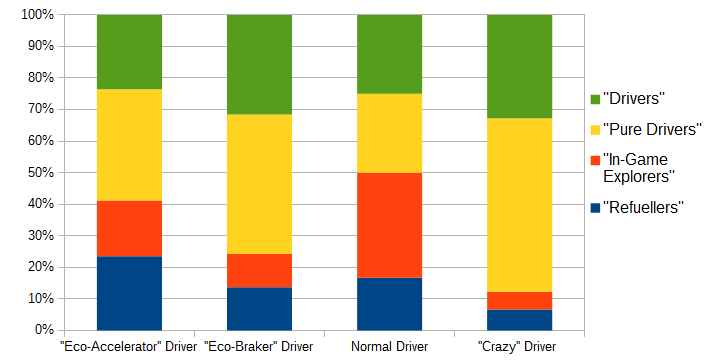
\includegraphics[width=.8\linewidth]{ijhcs14-img/cluster_activities_driver_types}
		\caption{Distribution of the activity clusters among users' driving profile.\label{fig:activity_driving}}
	\end{center}
\end{figure}


\subsection{Analysis of Users' Eco-Driving Evolution}
\label{subsec:eco-friendliness_over_time}

In this section, we aim to test the hypothesis that users become more eco-friendly drivers over time. This is an obvious assumption for an eco-driving interface.

\begin{figure}[!tb]
	\centering
	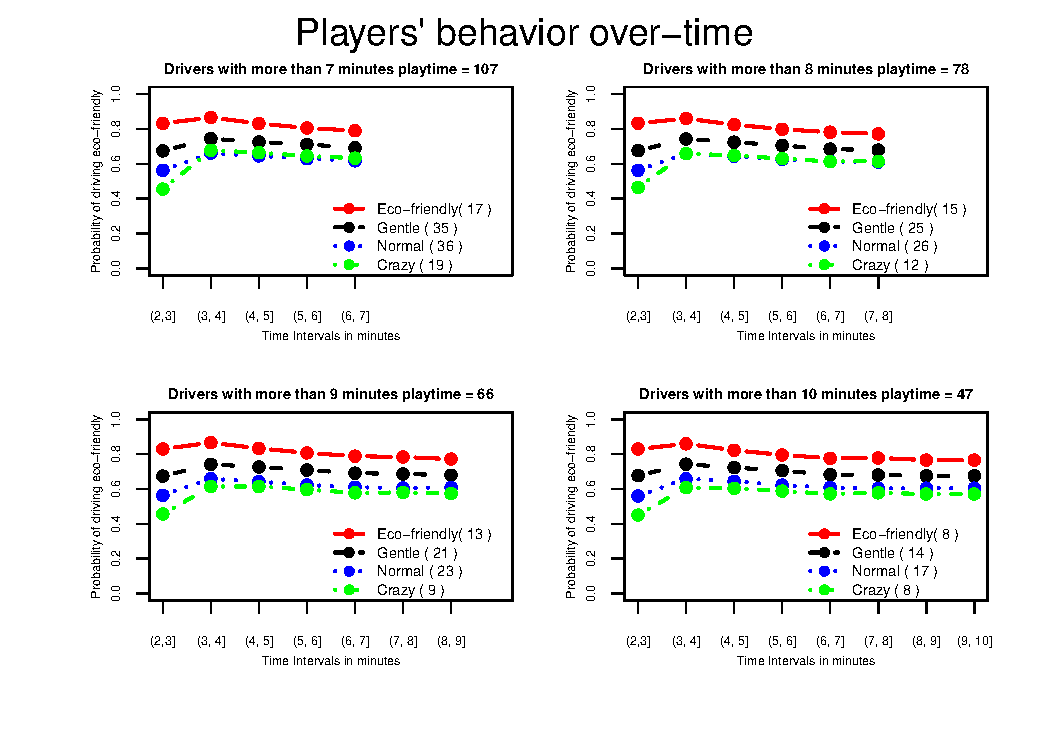
\includegraphics[width=1\linewidth]{ijhcs14-img/Evolution.pdf}
	\caption{Users' eco-driving behavior over time. \hl{PLEASE REMOVE THE BIG CAPTION FROM THE PICTURE; ALSO PLEASE INCREASE FONT SIZE OF X AND Y AXIS LABELS.}
}
	\label{fig:evolution}
\end{figure}

The approach is to first select the users who drove more than a certain amount of time and then to calculate the variation of the probabilities of them performing smooth acceleration in discrete uniform time-intervals.

To implement this approach, four different play-times are chosen: 7, 8, 9 and 10 minutes. Players who drove less than these times are filtered out. For the remaining players, driving behavior data for their entire driving duration is collected, except for the first two minutes, which is considered as training time.
%The rationale behind the choice of these playtimes is that we wanted a player to drive for a reasonably longer period so that their performance can be tested.
Then, for each group of players that correspond to a different play-time, clustering based on the probability of their jerk distribution (see Eq.~\ref{eq:factor-accel-slope}) is performed to create the driver types clusters after a formal train session of first two minutes ends. \hl{TO BE SURE: 2 MINS TRAINING TIME, THEN 2 MINUTES CLUSTERING TIME, AND THEN THE REST. RIGHT?}

Using the `elbow' heuristic to minimize the Sum of squares due to error (Equation \ref{eq:sse}), the appropriate number of clusters $k$ are found to be four.
These driver types are named as ``Eco-friendly'', ``Gentle'', ``Normal'' and ``Crazy''.\hl{PLEASE BRIEFLY EXPLAIN WHY THE NAMING IS DIFFERENT.} Figure~\ref{fig:evolution} shows: (1) four different types of drivers filtered according to their driving time; (2) the number of drivers in each group; (3) the distribution of users within the four clusters of driver types, and (4) the time-varying distribution of the eco-friendliness of different driver types.

 A total of 2045 users were selected.\hl{NOT SURE I UNDERSTAND. SELECTED FOR WHAT? IN THE FIGURE YOU HAVE 107+76+66+47. WHAT'S THE MEANING OF 2045?}
 
%%% This just seems repetition... 
%The players are filtered into \textit{four} groups according to their net driving time. For each group, the players are clustered into \textit{four} clusters after training their driving with the simulator for first two minutes. Then their probability of having smooth acceleration within a certain time interval is calculated. The graphs show that for all the four groups, the \emph{crazy} drivers tend to perform eco-friendlier over time and match those termed as \textit{gentle} post-training.

Figure~\ref{fig:evolution} shows that ``Gentle'' drivers dominate in all four clusters, whereas ``Crazy'' drivers have the smallest share. The share of "Gentle" drivers is 32.7\%, 32.05\%, 31.81\% and 29.78\% for the players who played more than 7 minutes, 8 minutes, 9 minutes and 10 minutes respectively, while the share of "Crazy" drivers is 17.75\%, 15.5\%, 13.6\% and 17\%. \hl{WHAT DOES "SHARE" MEAN. I DON'T SEE ANYTHING LIKE THIS IN THE FIGURE...I ONLY SEE NUMBER OF PLAYERS....}
The data shows that the order of share of players according to the driver-types across all the groups is:  "Crazy" \textless "Normal" \textless "Gentle" \textless "Eco-friendly". This suggests that after due to the result of training (done for first 2 minutes of playtime), only a few drivers continue to drive is least eco-friendly way.
\hl{PLEASE RE-WRITE }

To further analyze the multi-plot Figure~\ref{fig:evolution}, we set a convention to read it by row. For all the plots, it can be seen that the eco-friendliness of the ``Crazy'' drivers improves significantly over time and becomes comparable with that of the ``Normal'' drivers. The eco-friendliess of ``Gentle'' drivers also increases. However, even the the high-performance users, i.e., the "Eco-friendly" drivers continue to maintain their edge over other driver types, although their performance decreases over time. 

 One explanation is that users prioritize the quests. The nature of quests requires a player to accelerate and decelerate the car (to stop), which will increase the player's distribution in non-smooth acceleration zones. % this a fluctuation in eco-friendliness is quite likely.
 Another explanation could be fatigue. 
 
 It is interesting to notice that for all the four driver types across all the four groups, the peak improvement occurs between 3 minutes to 4 minutes of playtime. Here we would like to argue that this finding is correlated with the fact that the median time for performing two quests (i.e.~completing the engagement) is 4 minutes and players get paid only when they finish an engagement. \hl{PLEASE MAKE SURE THE 4 MINUTES MEDIAN IS CONSISTENT WITHIN THE PAPER.} Thus, it can be hypothesized that players' motivation to ``perform'' somewhat decreases once they get paid.
\hl{I DELETED THE TEXT FOR IN-GAME CURRENCY. THE RECEIVED CURRENCY FOR A DIFFERENT GAME, NOT ICO2.}

Overall, our results support the hypothesis that the players who drive less eco-friendly in the beginning of their play-time, improve their driving over time.



\section{Conclusions} \label{sec:conclusions}

\hl{I CHECKED THIS SECTION ONLY ROUGHLY.}

In this paper, we describe iCO$_2$, a game-like simulation platform for collecting large-scale driving behavior data and other data on users' in-game activities, such as upgrading the user's car, while offering a virtual environment for the practice of eco-driving. As a research tool, iCO$_2$ can be seen as a Human Computation system where humans provide driving behavior. This allows us to better understand how users interact with a game that motivates them to drive eco-friendly. In this way, our system is related to other activities aimed at attracting users' work, such as Games with a Purpose or crowdsourcing. The proposed version of iCO$_2$ extends the previous version \citep{prendingeroliveira2014} by a quest system and a ``garage`` to improve the capabilities of the player's vehicle.

The main technical contribution is our iCO$_2$ campaign. Since our simulation platform is developed as a mobile app, we could use a mobile games promoter to attract users to our game. Fortunately, data of more than 3000 users could be collected in about one week. We were interested both in results about eco-driving behavior and results about the usage of our system.

The campaign and its analysis is an important step towards understanding players of mobile games that have a `serious' aspect, such as sustainable behavior. The next is to use the information of player types (``Eco-Braker``, ``Crazy``, etc) and classify the user's behavior in real-time. This classification can be used to alert the user during the game.

Using the data, we tested the hypothesis that the players who appear to be less eco-friendly in the beginning of their play-time improve as they play further. The approach is to select the players who played more than a certain amount of time and calculate the variation of the probabilities of them having smooth acceleration in discrete uniform time-intervals.

Almost 20\% of the users continued to play the game after the required two quests were completed.
The usage data also revealed some interesting details about users' in-game behavior, such as play-state switching, transaction, car switching and car color switching.

Future work will also try to increase the re-playability of the game to be able collect data of users over time. This opens up entirely new ways of feedback mechanisms to users as we may learn the user's behavior and reactions.


\section{Acknowledgments}
We are grateful to Klaus Bruegmann for coordinating the game design of iCO$_2$, and Tristan Imbert and Kugamoorthy Gajananan for helping with the preparation of the campaign.
This work is partly supported by a Kaken B grant from the Japan Society for the Promotion of Science and by Portugal’s Fundação para a Ciência e a Tecnologia, under project
PEst-OE/EEI/LA0021/2013


%% The Appendices part is started with the command \appendix;
%% appendix sections are then done as normal sections

\section*{References}
\bibliographystyle{elsarticle-harv}
\bibliography{ijhcs-2014}

%\appendix

%\section{Additional Tables}\label{app:tables}
%This section contains additional tables of our findings.

%sorted table
%\begin{table}[!h]
%\renewcommand*{\arraystretch}{1.4}
%\caption{Example of driving behavior data.}
%\begin{center}
%\begin{tabular}{c|c|c|c}
%Timestamp & Position $X$ & Position $Y$ & Position $Z$ \\
%\hline
%1 & 299.5657 & 1.241717 & 0.065165 \\

%2 & 299.2299 & 3.699343 & 0.065120  \\

%3 & 299.2299 & 3.699343 & 0.06512 \\

%4 & 298.8777 & 6.260628 & 0.066202 \\

%5 & 298.8777 & 6.260628 & 0.066202 \\

%6 & 298.7033 & 7.509112 & 0.066517 \\

%\ldots &  \ldots & \ldots & \ldots \\

%2635 & 300.7204	& $-$6.95397 & 0.064981 \\

%2636 & 300.8299	& $-$7.72201 & 0.065020 \\

%2637 & 300.8299	& $-$7.72201 & 0.065020 \\

%2638 & 301.0301	& $-$9.08316 & 0.065068 \\

%2639 & 301.1052	& $-$9.57525 & 0.065062
%\end{tabular}
%\end{center}
%\label{T:drivingdata}
%\end{table}


%sorted table
%\begin{table}[!h]
%\renewcommand*{\arraystretch}{1.4}
%\caption{Acceleration ranges and example values of user in those ranges.}
%\begin{center}
%\begin{tabular}{c|c}
%Range & Value \\
%\hline
%[$-$infinite, $-$5.00] & 15.5022 \\

%[$-$5.00, $-$4.00]	& 5.0364 \\

%[$-$4.00, $-$3.00]	& 11.1235 \\

%[$-$3.00, $-$2.00]	& 4.0027 \\

%[$-$2.00, $-$1.00]	& 21.825 \\

%[$-$1.00, 0.00]	& 20.3731 \\

%[0.00, 1.00]	& $-$0.19349 \\

%[1.00, 2.00]	& $-$0.01021 \\

%[2.00, 3.00]	& 3.7433 \\

%[3.00, 4.00]	& 3.5839 \\

%[4.00, 5.00]	& 4.5173 \\

%[5, +infinite]	& 13.6953 \\
%\end{tabular}
%\end{center}
%\label{T:acceleration}
%\end{table}


%sorted table
%\begin{table} [!h]
%\renewcommand*{\arraystretch}{1.4}
%\caption{Velocity ranges and example values of user in those ranges.}
%\begin{center}
%\begin{tabular}{c|c}
%Range & Value \\
%\hline
%[0.00, 30.00] &	     0.113387 \\

%[30.00, 60.00] &	$-$0.03678 \\

%[60.00, 90.00] &	$-$0.12182 \\

%[90.00, 120.00] &	$-$0.05689 \\

%[120,  +infinite] &	$-$0.05036
%\end{tabular}
%\end{center}
%\label{T:velocity}
%\end{table}




%\section{Additional Charts}
%% \label{}
%This section contains additional charts from our campaigns.

%\begin{figure}[ht]
% \centering
% \subfigure[Campaign requirements]{
%  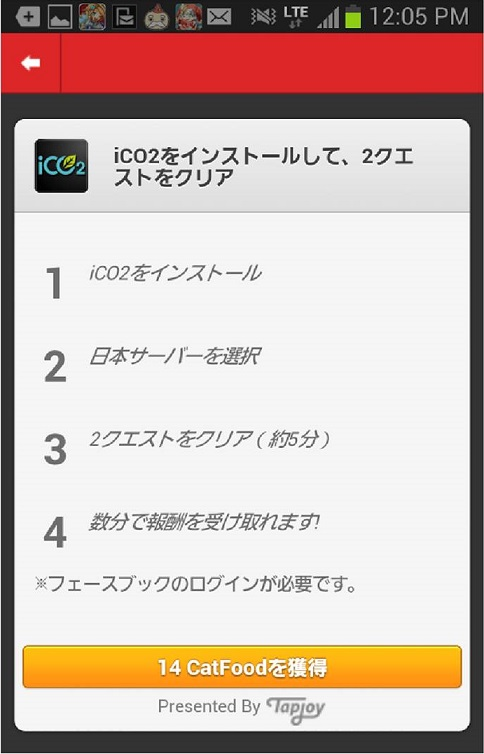
\includegraphics[scale=0.5]{ijhcs14-img/tapjoy}
%   \label{fig:requirements}
%   }
% \subfigure[Display of iCO$_2$ in game list]{
%  
\includegraphics[scale=0.55]{ijhcs14-img/gamelist}
%   \label{fig:gamelist}
%   }
% \label{fig:tapjoy}
% \caption[Tapjoy campaign]{%
%  Tapjoy campaign
%  }
%\end{figure}


%\clearpage % Start a new page

%\setstretch{1.5} % Set the line spacing to 1.5, this makes the following tables easier to read

%\section{Abbreviations}\label{app:abbreviations}
%\listofsymbols{ll} % Include a list of Abbreviations (a table of two columns)
%\begin{tabular}{ l | l }
%	\textbf{3D} & \textbf{3} \textbf{D}imensional \\
%	\textbf{DiVE} & \textbf{Di}stributed \textbf{V}irtual \textbf{}Environments \\
%	\textbf{ESP} & \textbf{E}xtra\textbf{s}ensory \textbf{P}erception  \\
%   \textbf{GWAP} & \textbf{G}ames \textbf{W}ith \textbf{A} \textbf{P}urpose \\
%    \textbf{iOS} & \textbf{i}Phone \textbf{O}perating \textbf{S}ystem \\
%    \textbf{MMO} & \textbf{M}assive \textbf{M}ultiplayer \textbf{O}nline \\
%    \textbf{MMOG} & \textbf{M}assive \textbf{M}ultiplayer \textbf{O}nline \textbf{G}ame \\
%    \textbf{SSE} & \textbf{S}um of \textbf{S}quares due to \textbf{E}rror \\
%\end{tabular}


%\begin{figure}[htb]
%\begin{center}
%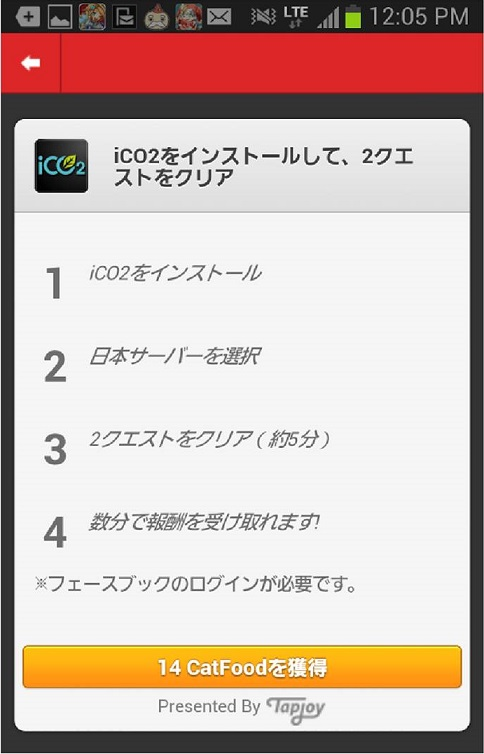
\includegraphics[width=.4\linewidth]{ijhcs14-img/tapjoy}
%\caption{Requirements of the Tapjoy campaign.\label{fig:requirements}}
%\end{center}
%\end{figure}

%\begin{figure}[htb]
%\begin{center}
%
\includegraphics[width=.4\linewidth]{ijhcs14-img/gamelist}
%\caption{Presentation of iCO$_2$ campaign in game list.\label{fig:gamelist}}
%\end{center}
%\end{figure}

\appendix
\section{Play Sessions}
\begin{figure}[htb]
	\begin{center}
		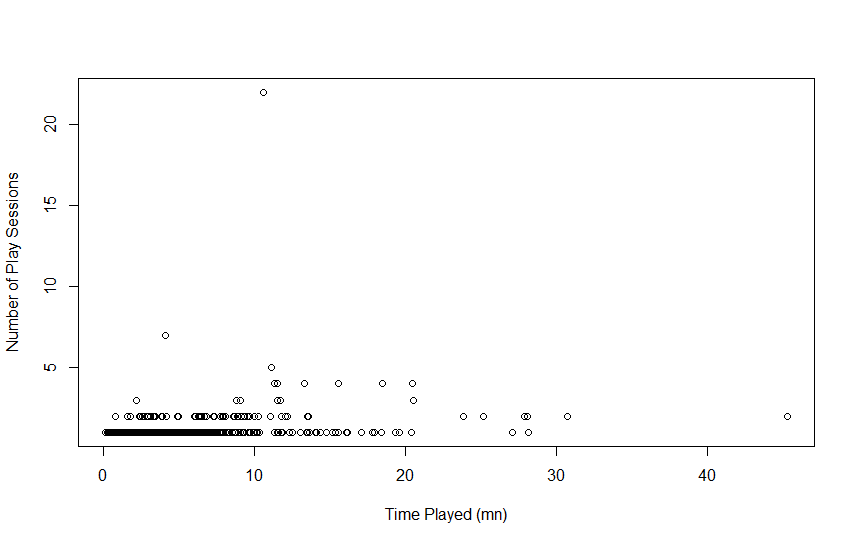
\includegraphics[width=.8\linewidth]{ijhcs14-img/playsessions_europe}
		\caption{Distribution of play sessions by total play time for Europe.\label{fig:playtime_e}}
	\end{center}
\end{figure}

\begin{figure}[htb]
	\begin{center}
		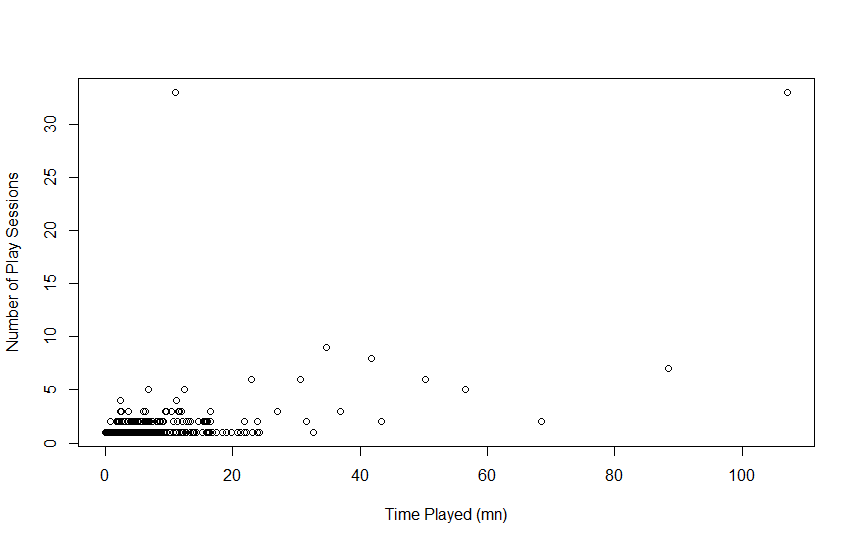
\includegraphics[width=.8\linewidth]{ijhcs14-img/playsessions_asia}
		\caption{Distribution of play sessions by total play time for Asia.\label{fig:playtime_as}}
	\end{center}
\end{figure}

\begin{figure}[htb]
	\begin{center}
		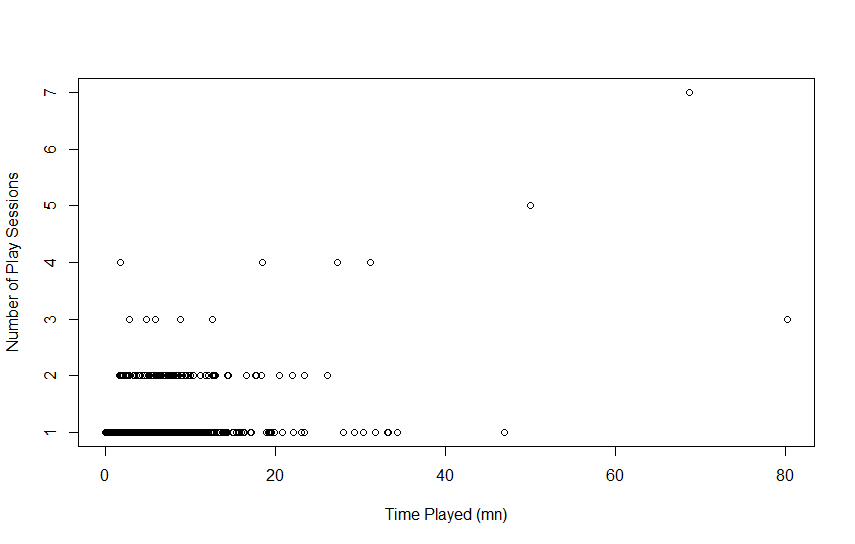
\includegraphics[width=.8\linewidth]{ijhcs14-img/playsessions_america}
		\caption{Distribution of play sessions by total play time for America.\label{fig:playtime_a}}
	\end{center}
\end{figure}

%\section{Driving Behavior and Chosen Car Color}
%
%\begin{table}[!h]
%	\renewcommand*{\arraystretch}{1.2}
%	\caption{Joint distribution of player profile and chosen car color for Europe.}
%	\begin{center}
%		\begin{tabular}{c|c|c|c|c}
%			Color	& Cluster 1 &	Cluster 3 &	Cluster 4 &	Cluster 2 	\\
%			Blue &	0.091 &	0.045 &	0.000 &	0.045 \\
%			Gray &	0.000 &	0.000 &	0.000 &	0.091  \\
%			Green &	0.000 & 0.000 &	0.091 &	0.045  \\
%			Red &	 0.000 &	 0.000 &	0.227 & 0.227  \\
%			White &	0.000 &	0.000 &	0.091 &	0.045  \\
%			Yellow &	0.000 &	0.000 &	0.000 & 0.000 \\
%		\end{tabular}
%	\end{center}
%	\label{T:colour_correlation_europe}
%\end{table}
%
%\begin{table}[!h]
%	\renewcommand*{\arraystretch}{1.2}
%	\caption{Joint distribution of player profile and chosen car color for Asia.}
%	\begin{center}
%		\begin{tabular}{c|c|c|c|c}
%			Color	& Cluster 1 &	Cluster 3 &	Cluster 4 &	Cluster 2 	\\
%			Blue &	0.033 &	0.067 &	0.000 &	0.067 \\
%			Gray &	0.000 &	0.033 &	0.000 &	0.133  \\
%			Green &	0.100 & 0.000&	0.033 &	0.167  \\
%			Red &	 0.000 &	 0.000 &	0.100 & 0.167  \\
%			White &	0.000 &	0.000 &	0.000 &	0.067  \\
%			Yellow &	0.000 &	0.033 &	0.000 & 0.000 \\
%		\end{tabular}
%	\end{center}
%	\label{T:colour_correlation_asia}
%\end{table}
%
%
%\begin{table}[!h]
%	\renewcommand*{\arraystretch}{1.2}
%	\caption{Joint distribution of player profile and chosen car color for America.}
%	\begin{center}
%		\begin{tabular}{c|c|c|c|c}
%			Color	& Cluster 1 &	Cluster 3 &	Cluster 4 &	Cluster 2 	\\
%			Blue &	0.043 &	0.000 &	0.130 &	0.043 \\
%			Gray &	0.000 &	0.000 &	0.000 &	0.0436  \\
%			Green &	0.000 & 0.000 &	0.130&	0.087  \\
%			Red &	 0.000 &	 0.043&	0.217 & 0.174  \\
%			White &	0.000 &	0.000 &	0.000 &	0.043  \\
%			Yellow &	0.000&	0.000 &	0.043 & 0.000 \\
%		\end{tabular}
%	\end{center}
%	\label{T:colour_correlation_america}
%\end{table}

\end{document}
%%% Local Variables:
%%% coding: euc-japan 